\documentclass[11pt,a4paper]{article}
\usepackage[utf8]{inputenc}
\usepackage[T1]{fontenc}
\usepackage{amsfonts}
\usepackage[french]{babel}
\frenchbsetup{StandardLists=true} % à inclure si on utilise \usepackage[francais]{babel}
\usepackage{enumitem}
\usepackage{amssymb}
\usepackage{amsmath}
\usepackage[left=2cm,right=2cm,top=2cm,bottom=2cm]{geometry}
\usepackage{multirow}
\usepackage[dvipsnames]{xcolor}

\usepackage[T1]{fontenc}
\usepackage{fouriernc}
\usepackage{graphicx}

\usepackage{setspace}
\singlespacing

\usepackage{pstricks}
\usepackage{xkeyval}
\usepackage{pst-labo}


\usepackage{multicol}
\usepackage{caption}
\usepackage{fancyhdr}
\pagestyle{fancy}
\renewcommand\headrulewidth{1pt}
\fancyhead[L]{Lycée Denis Diderot }
\fancyhead[R]{Classe de Terminale}
\setcounter{page}{6}\fancyfoot[C]{page \thepage}
\fancyfoot[R]{Année 2025 2026}
\fancyfoot[L]{Alexis RUIZ}
\usepackage{multirow,tabularx,booktabs}
\newcommand{\cadreblanc}[1]{%
\medskip\framebox[\linewidth][c]{%
\rule{0mm}{#1mm}}\par
\medskip}

\usepackage{awesomebox}
\setlength{\aweboxvskip}{0mm}
\usepackage{pifont}
\usepackage{chemmacros}
\chemsetup{modules=all}

\renewcommand{\arraystretch}{2}
\newcommand*\acocher{\quitvmode{\fboxsep0pt \fboxrule0.8pt \fbox{\vrule height1.8ex depth.1ex width0pt \vrule height0pt depth0pt width1.9ex }}}

\newcommand{\defproblem}{\awesomebox[black]{2pt}{\rotatebox{90}{\large{\textbf{Problématique}}}}{black}}
\newcommand{\defconclusion}{\awesomebox[black]{2pt}{\rotatebox{90}{\Large{\textbf{Conclusion}}}}{black}}
\newcommand{\defbox}{\awesomebox[black]{2pt}{
\includegraphics[scale=0.5]{images/appel exam.png}}{black}}
\newcommand{\ecrire}{\awesomebox[black]{2pt}{\faEye}{black}}
\frenchbsetup{StandardLists=true}
\begin{document}





\ding{204} \textbf{Couple redox } 

\ecrire{\fbox{
\begin{minipage}{14cm}{
\textbf{ }\\
\vspace{9cm}
}

\end{minipage}
}}
\vspace {0.5cm}

\ding{205}\textbf{~~Classification } Les couples redox sont classées d'après leur pouvoir oxydant ( et donc réducteur aussi ) dans la classification électrochimique des métaux ci-dessous.
\begin{center}
\fbox{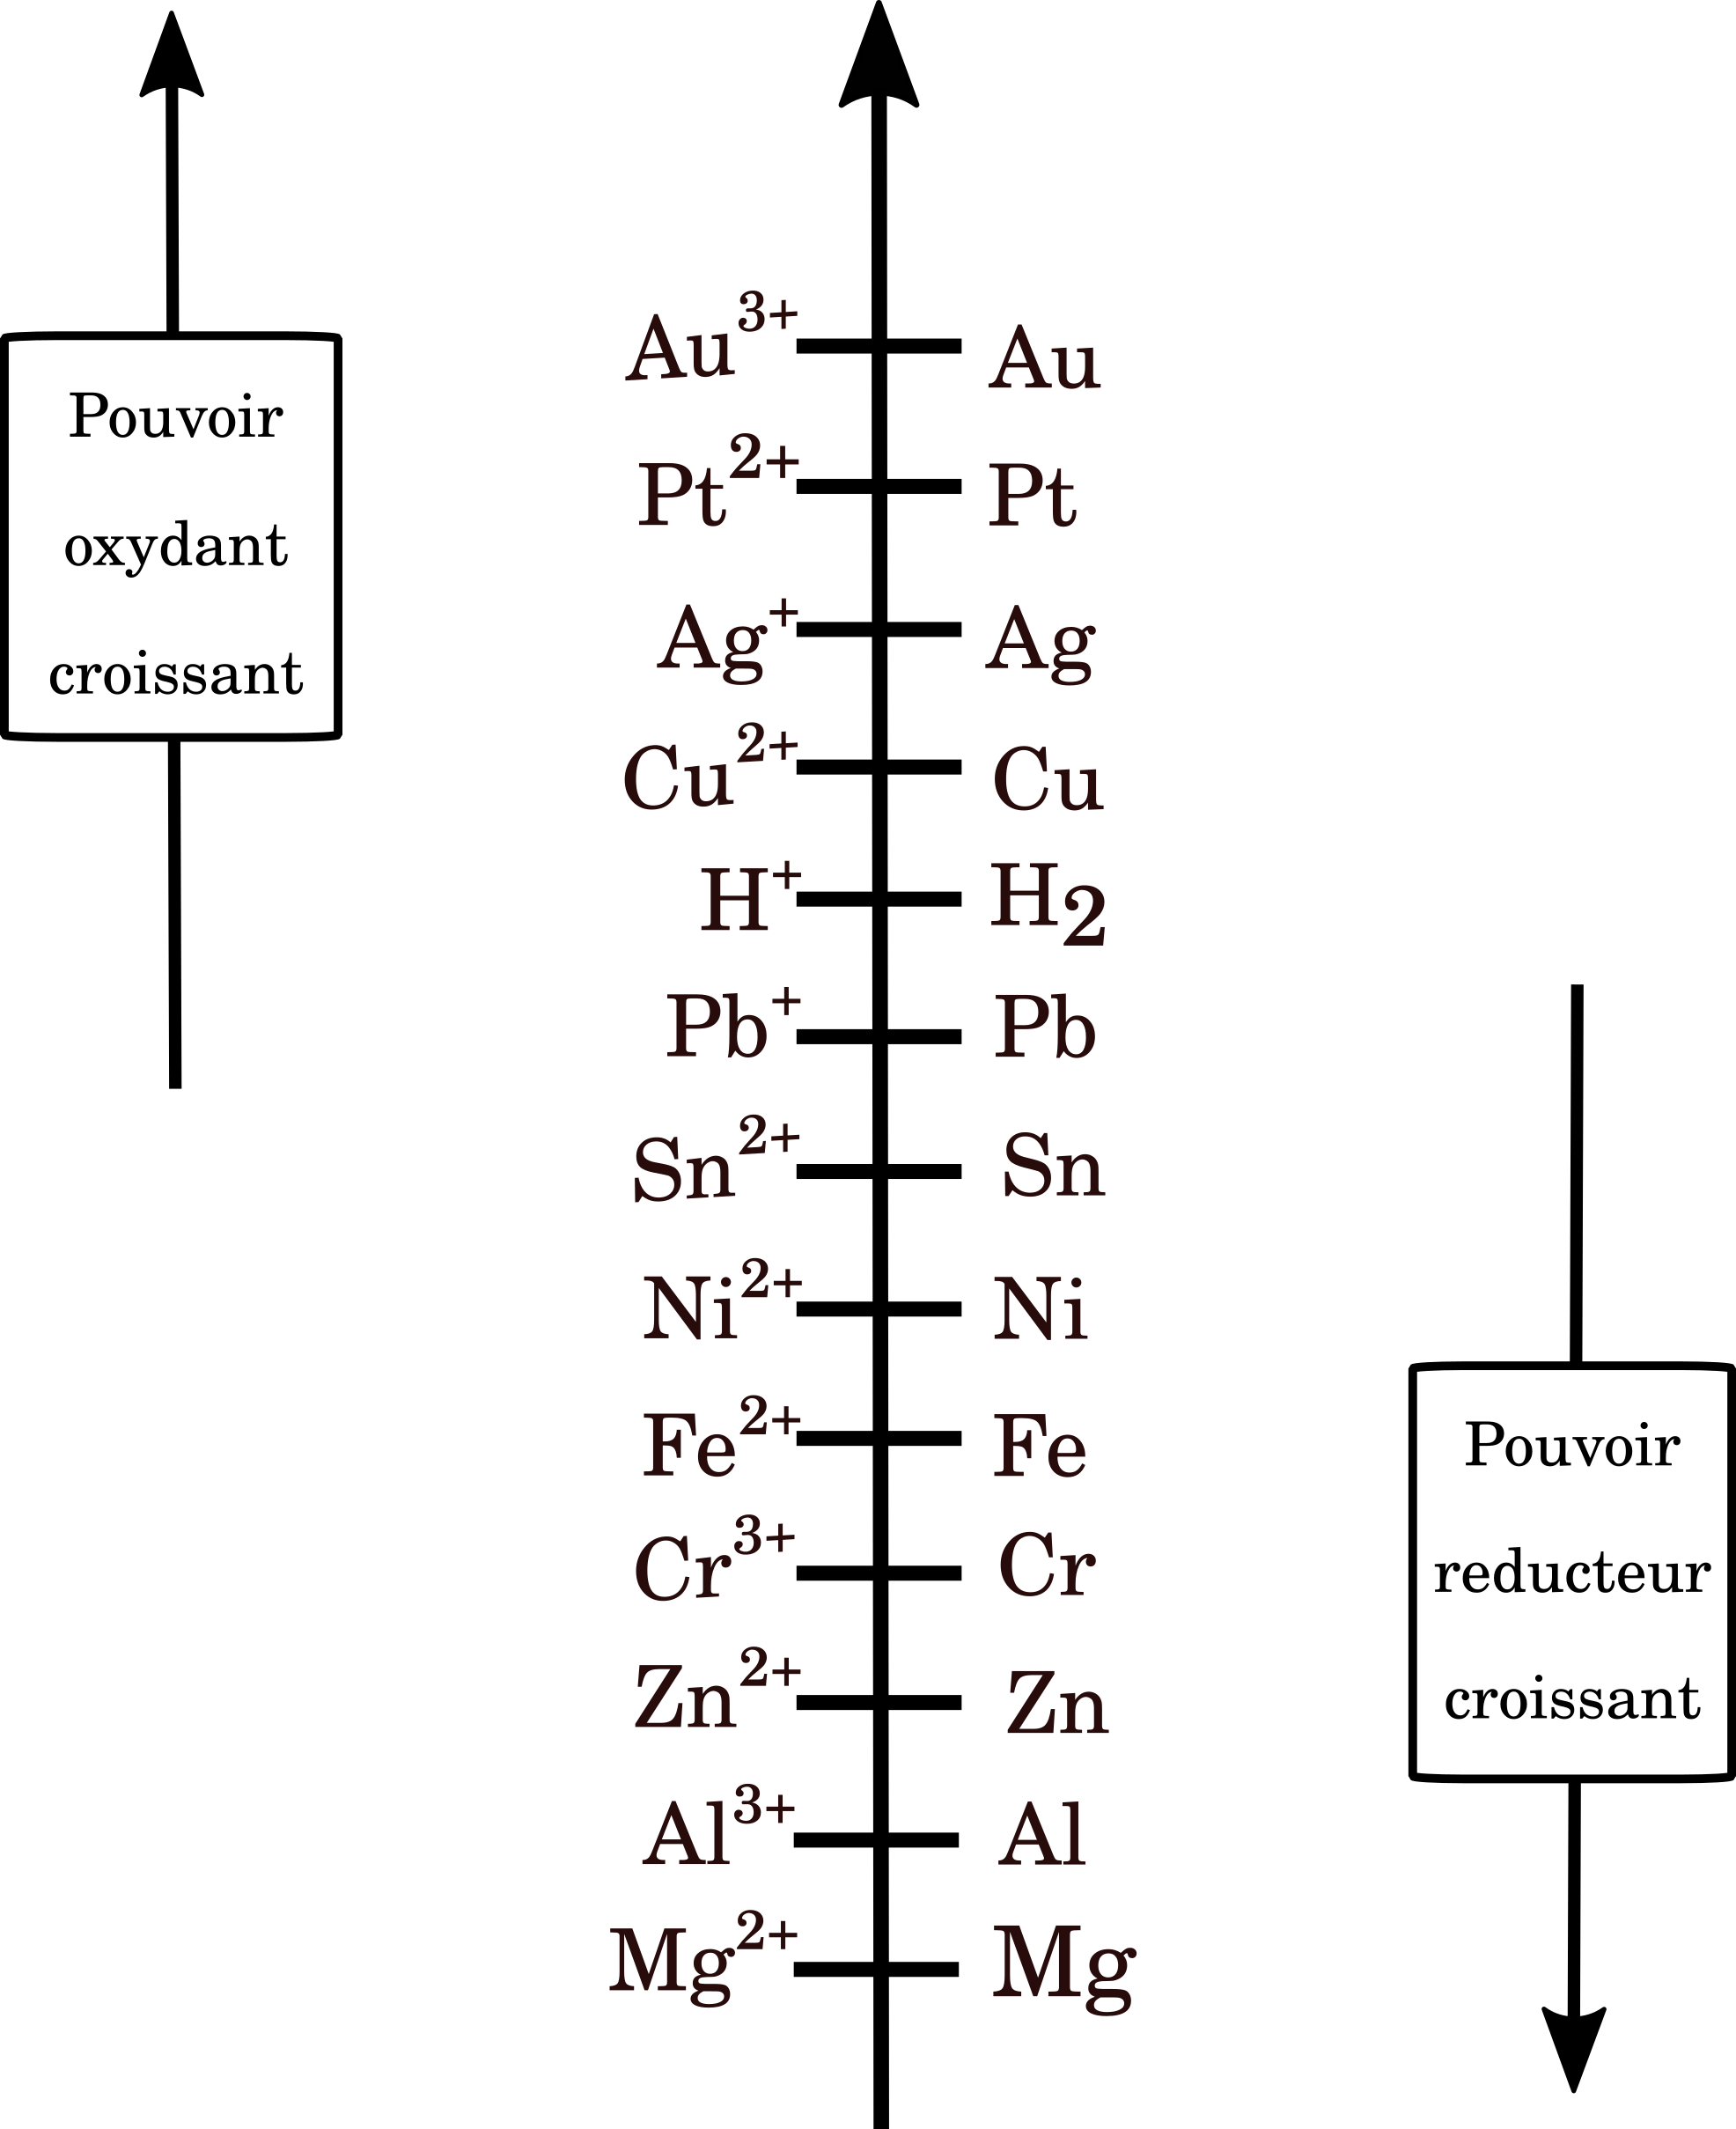
\includegraphics[scale=0.5]{images/classification.png} }
\end{center}

\vspace {0.5cm}

\ding{206}\textbf{~~Règle du gamma}
\begin{itemize}
\item Elle permet d'expliquer pourquoi la réaction d'oxydoréduction se réalise dans le cas d'une lame de fer dans des ions \ch{Cu\pch[2]} et ne se réalise pas dans le cas d'une lame de Cu dans des ions \ch{Fe\pch[2]}. 
\item Elle est un moyen rapide pour savoir quelle réaction se produit spontanément.
\end{itemize}

\newpage

\textbf{Exemple :} On trempe une lame de zinc (Zn) dans une solution contenant des ions argent (\ch{Ag\pch[]})



\begin{figure}[h]
\begin{minipage}{0.4\textwidth}
\begin{center}
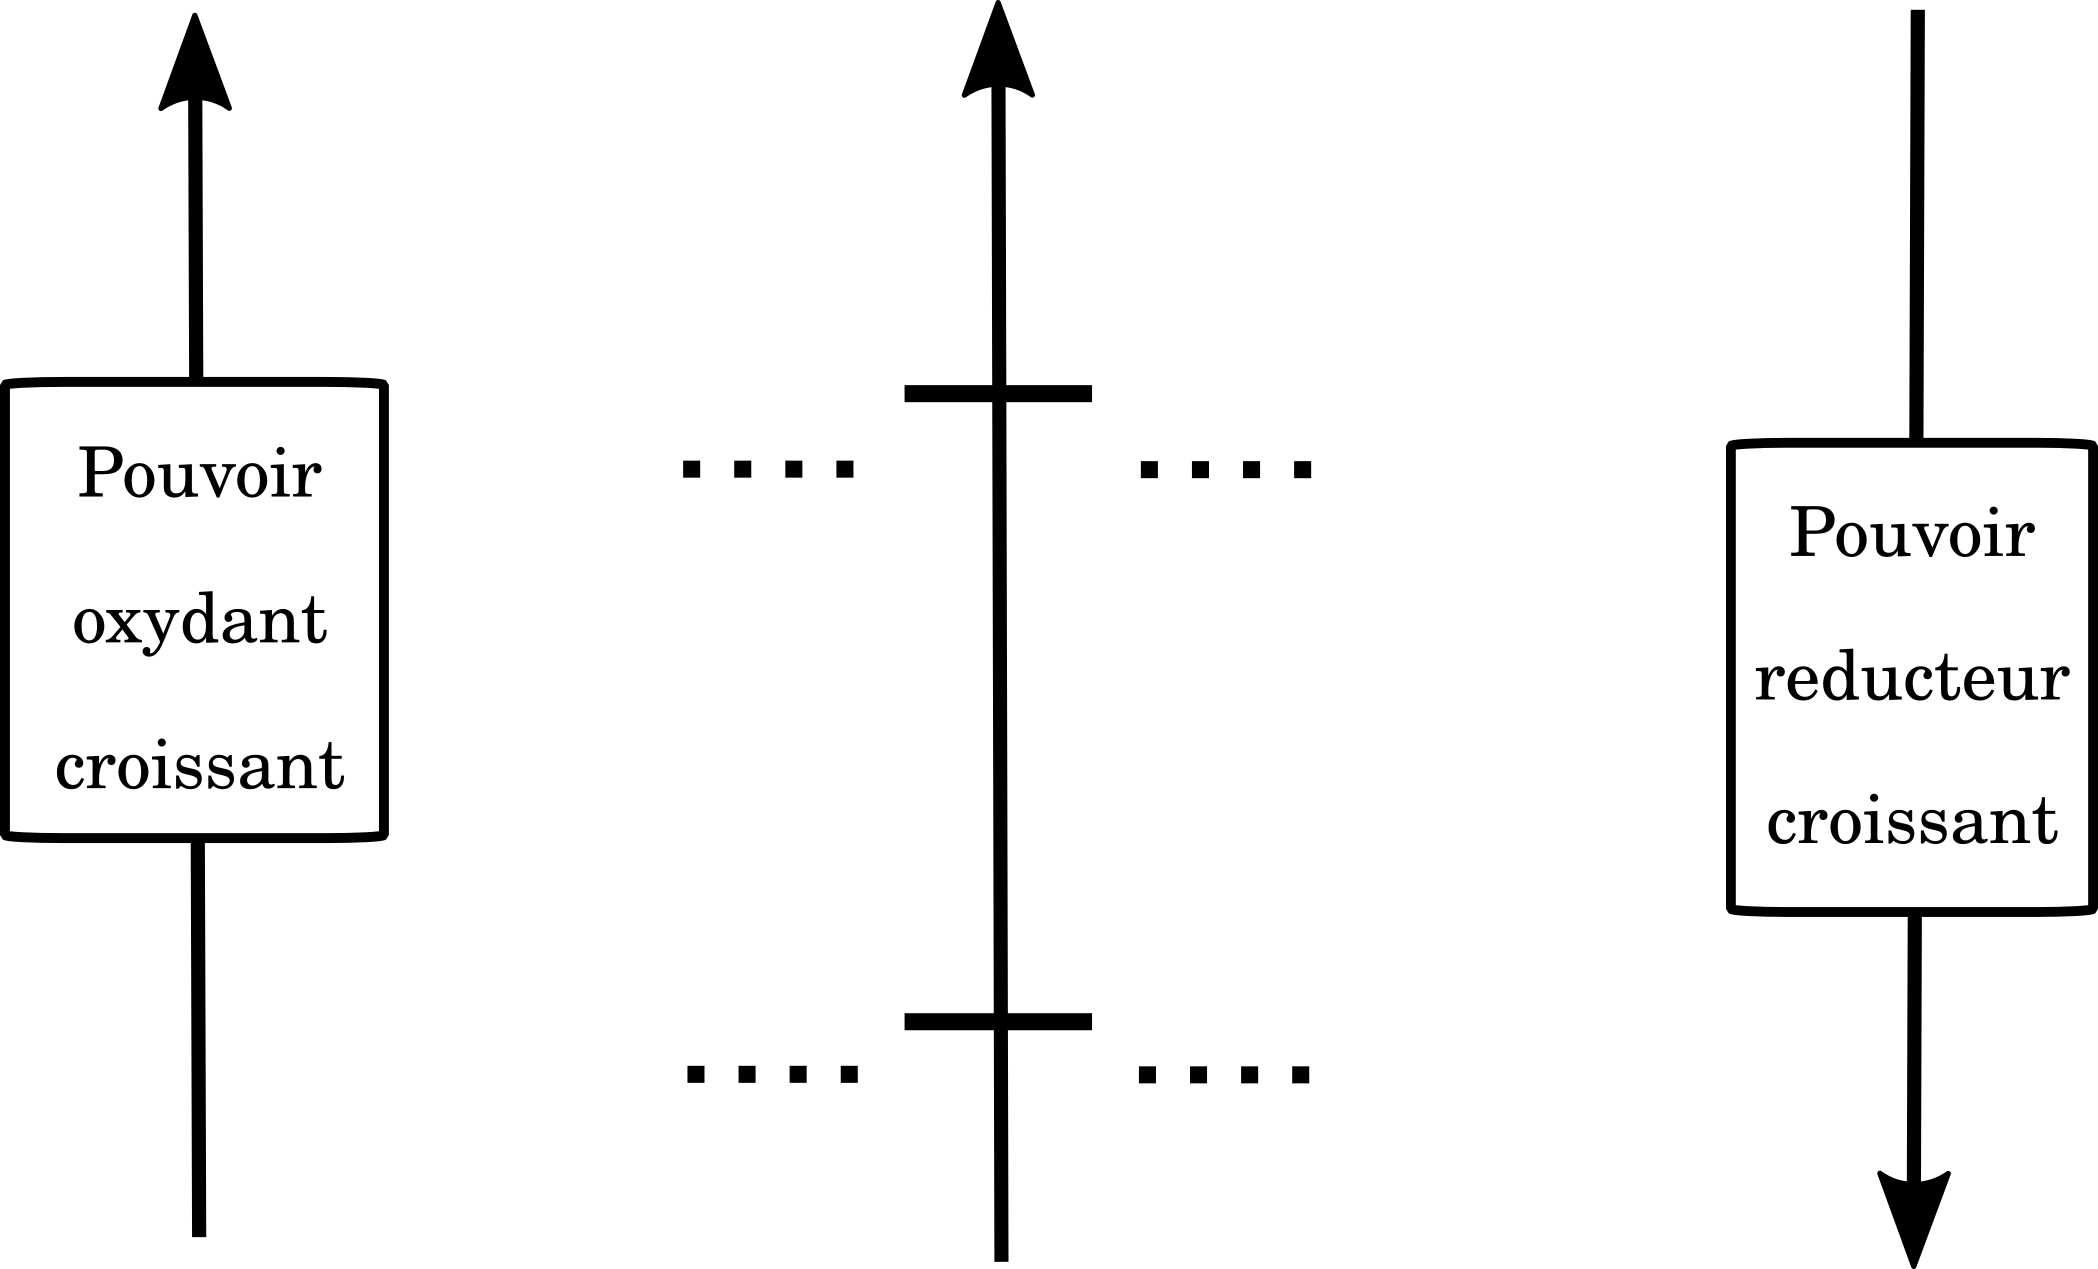
\includegraphics[scale=0.30]{images/classification 2 elements.png}
\end{center}
\end{minipage}%
\begin{minipage}{0.6\textwidth}
1. En utilisant la classification (page~~6) placer les couples redox \ch{Ag\pch[]}/ Ag et \ch{Zn\pch[2]}/Zn. \\

2. Tracer sur l'échelle le gamma. \\

\end{minipage}
\end{figure}
3. La réaction peut – elle avoir lieu ?\\

...............................................................................................................\\

4. Écrire les deux demi équations correspondantes à cette réaction. \\
\begin{center}
\LARGE\fbox{$~~~~~~ ~~\longrightarrow~~~~~~~~+ ~~~~~~~~~~ $}\\[3mm]
\fbox{$~~~~~~ ~~+ ~~~~~~~ ~~\longrightarrow ~~~~~~ ~~$}\\
\end{center}
\normalsize
5. Écrire l'équation de la réaction. \\
\begin{center}
\LARGE\fbox{$~~~~~~ ~~+ ~~~~~~ ~~ \longrightarrow ~~~~~~ ~~+ ~~~~~~ ~~ $}\\
\end{center}

\textbf{Exercice :} On trempe une bague en argent (Ag) dans une solution contenant des ions or (\ch{Au\pch[3]})



\begin{figure}[h]
\begin{minipage}{0.4\textwidth}
\begin{center}
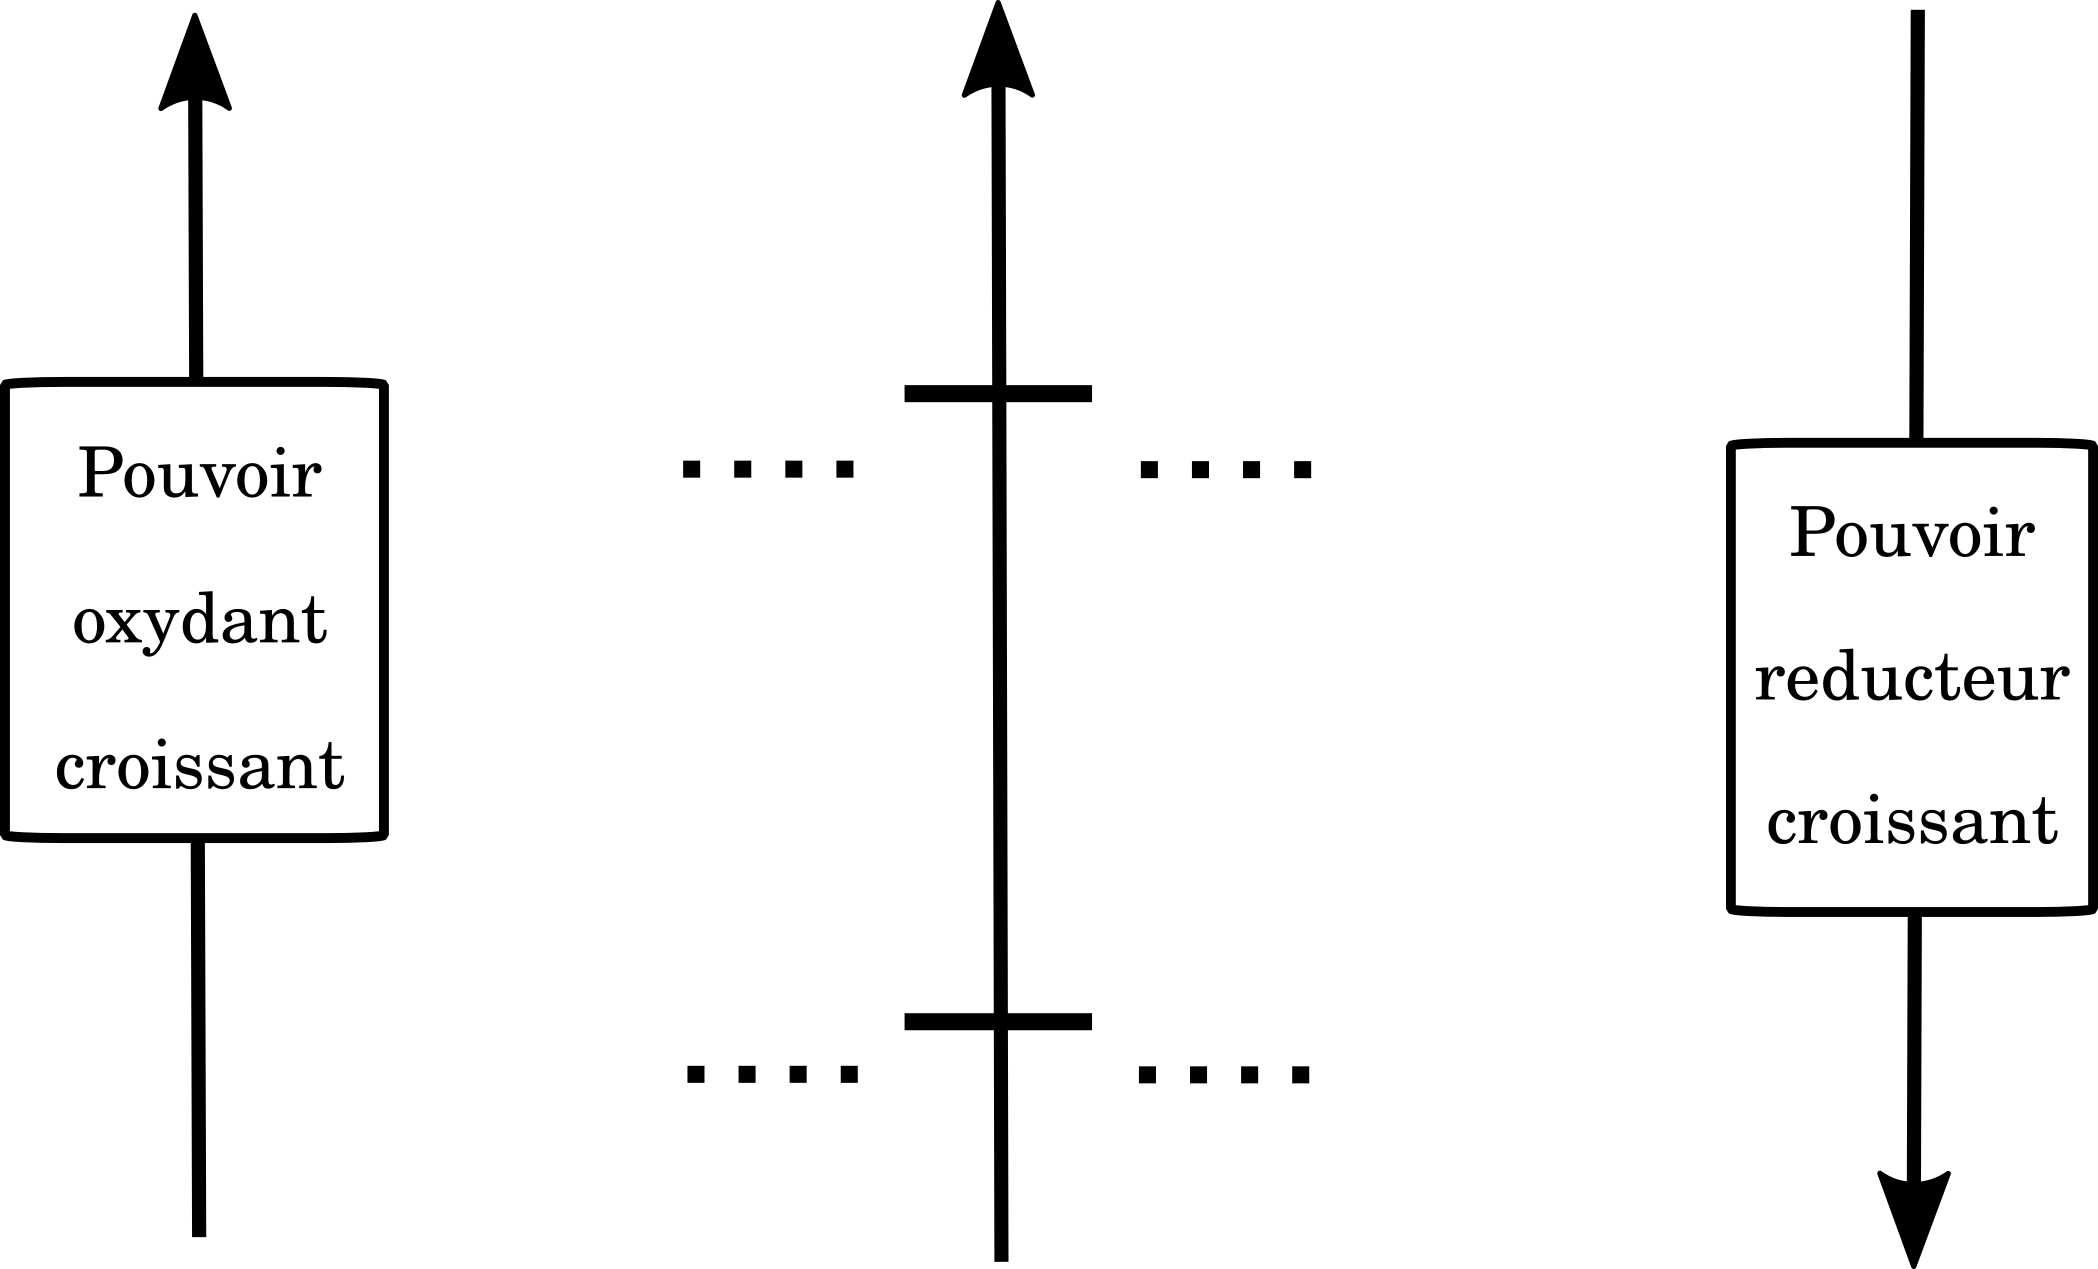
\includegraphics[scale=0.30]{images/classification 2 elements.png}
\end{center}
\end{minipage}%
\begin{minipage}{0.6\textwidth}
1. En utilisant la classification (page~~6) placer les couples redox \ch{Ag\pch[]}/ Ag et \ch{Au\pch[3]}/Au. \\

2. Tracer sur l'échelle le gamma. \\

\end{minipage}
\end{figure}
3. La réaction peut – elle avoir lieu ?\\

...............................................................................................................\\

4. Écrire les deux demi équations correspondantes à cette réaction. \\
\begin{center}
\LARGE\fbox{$~~~~~~ ~~\longrightarrow~~~~~~~~+ ~~~~~~~~~~ $}\\[3mm]
\fbox{$~~~~~~ ~~+ ~~~~~~~ ~~\longrightarrow ~~~~~~ ~~$}\\
\end{center}
\normalsize
5. Écrire l'équation de la réaction. \\
\begin{center}
\LARGE\fbox{$~~~~~~ ~~+ ~~~~~~ ~~ \longrightarrow ~~~~~~ ~~+ ~~~~~~ ~~ $}\\
\end{center}
\end{document}